\documentclass{article}
\begin{document}
\subsection{Copying the files using MTP}
The following procedure demonstrates how to copy files using MTP:
\begin{itemize}
	\item APP3.x comes with the preloaded MTP firmware update package.
	\item Refer to section \ref{SwitchModes} to switch to MTP mode
	\item The device will enumerate as an MTP device with name "Application Board 3.x". Click on it and select the "W25M02 External Memory"
	\item The device will list all the available files and all required files can be copied.
\end{itemize}

\begin{figure}[H]
	\begin{center}
		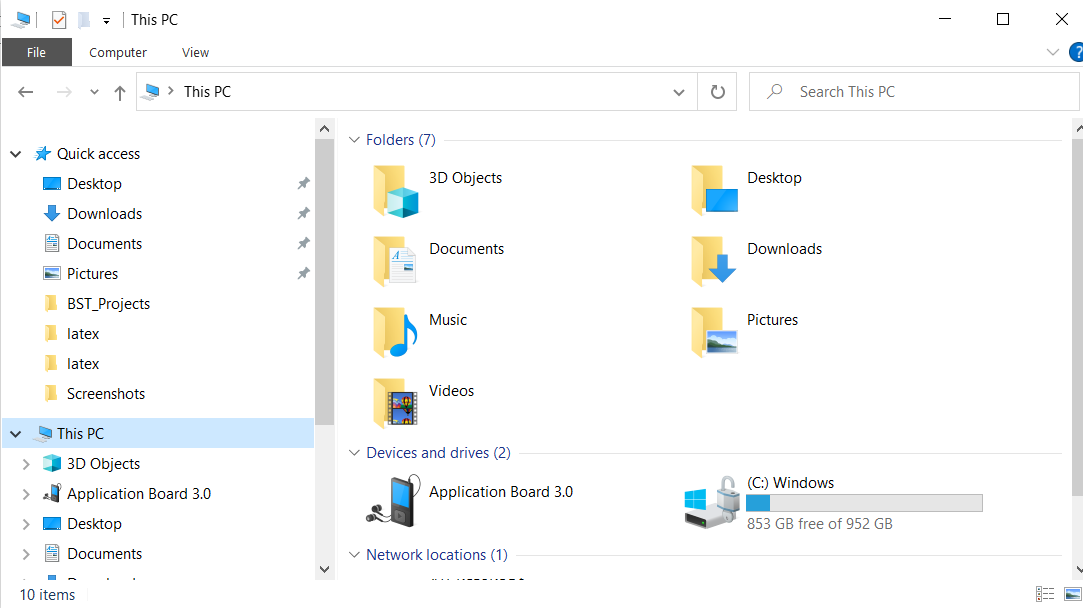
\includegraphics[width=0.7\textwidth]{coinesAPI_images/MTP_windows.png}
		\caption{Copy data log files to the PC over USB MTP}
	\end{center}
\end{figure}

\newpage

\end{document}